% !TEX root = main.tex

\section{Models}

\subsection{Logic Tensor Network (LTN)}

multilayer perceptron (MLP). The key differencen is that the first layer is not linear layer but bilinear layer.

\begin{figure}
    \centering
    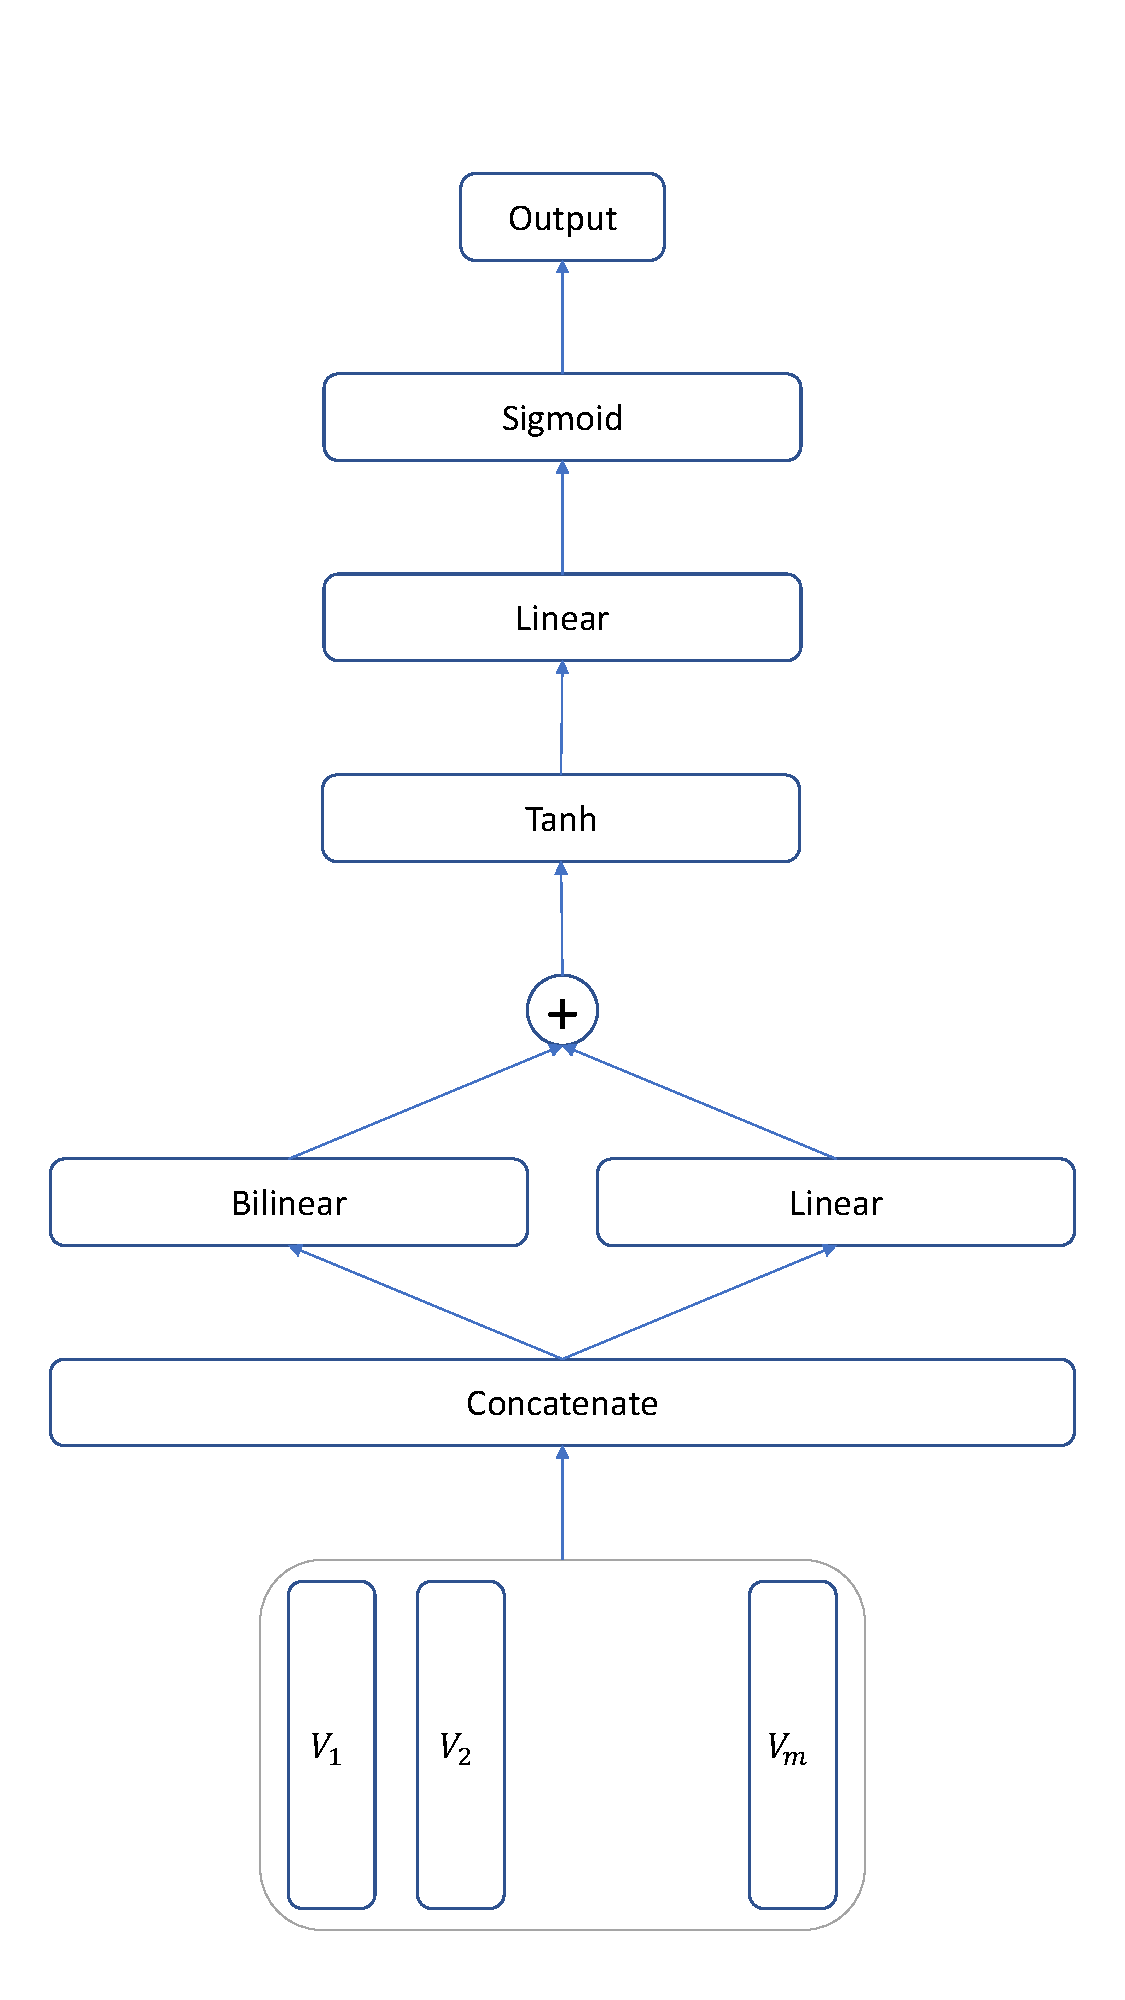
\includegraphics[width=.4\textwidth]{img/Predicate.pdf}
    \caption{Model for Predicate}
    \label{fig:LTN_predicate}
\end{figure}

\subsection{Convolutional Logic Tensor Network (CLTN)}

The model in original LTN is based on classical neural networks. However, recent development on deep learning shows that convolutional neural network (CNN) has more powerful ability. That makes us to extend LTN with CNN.

Here we first follow up the implementation of $G(c)$, $G(f)$, and $G(\phi)$. However, we tend to use Convolutional Neural Network to implement $G(p)$.

First we need to construct the input matrix with the $v_1,v_2,\dots,v_m$. From LTN model, we learned that the bilinear manipulation is critical to get a good performance. Here we construct this bilinear function directly using input vectors of constants. That is, suppose we get $m$ vectors called $x=[v_1,\dots,v_m]$, then $x\in \mathbb{R}^{k\times m}$, where $k$ is the dimension of constant vectors. Therefore, $x^Tx \in \mathbb{R}^{m\times m}$ a squre matrix, which can be treated as a 1-channel image.

The following step is trivial and the model is illustrated in Figure \ref{fig:CLTN_predicate}

\begin{figure}
    \centering
    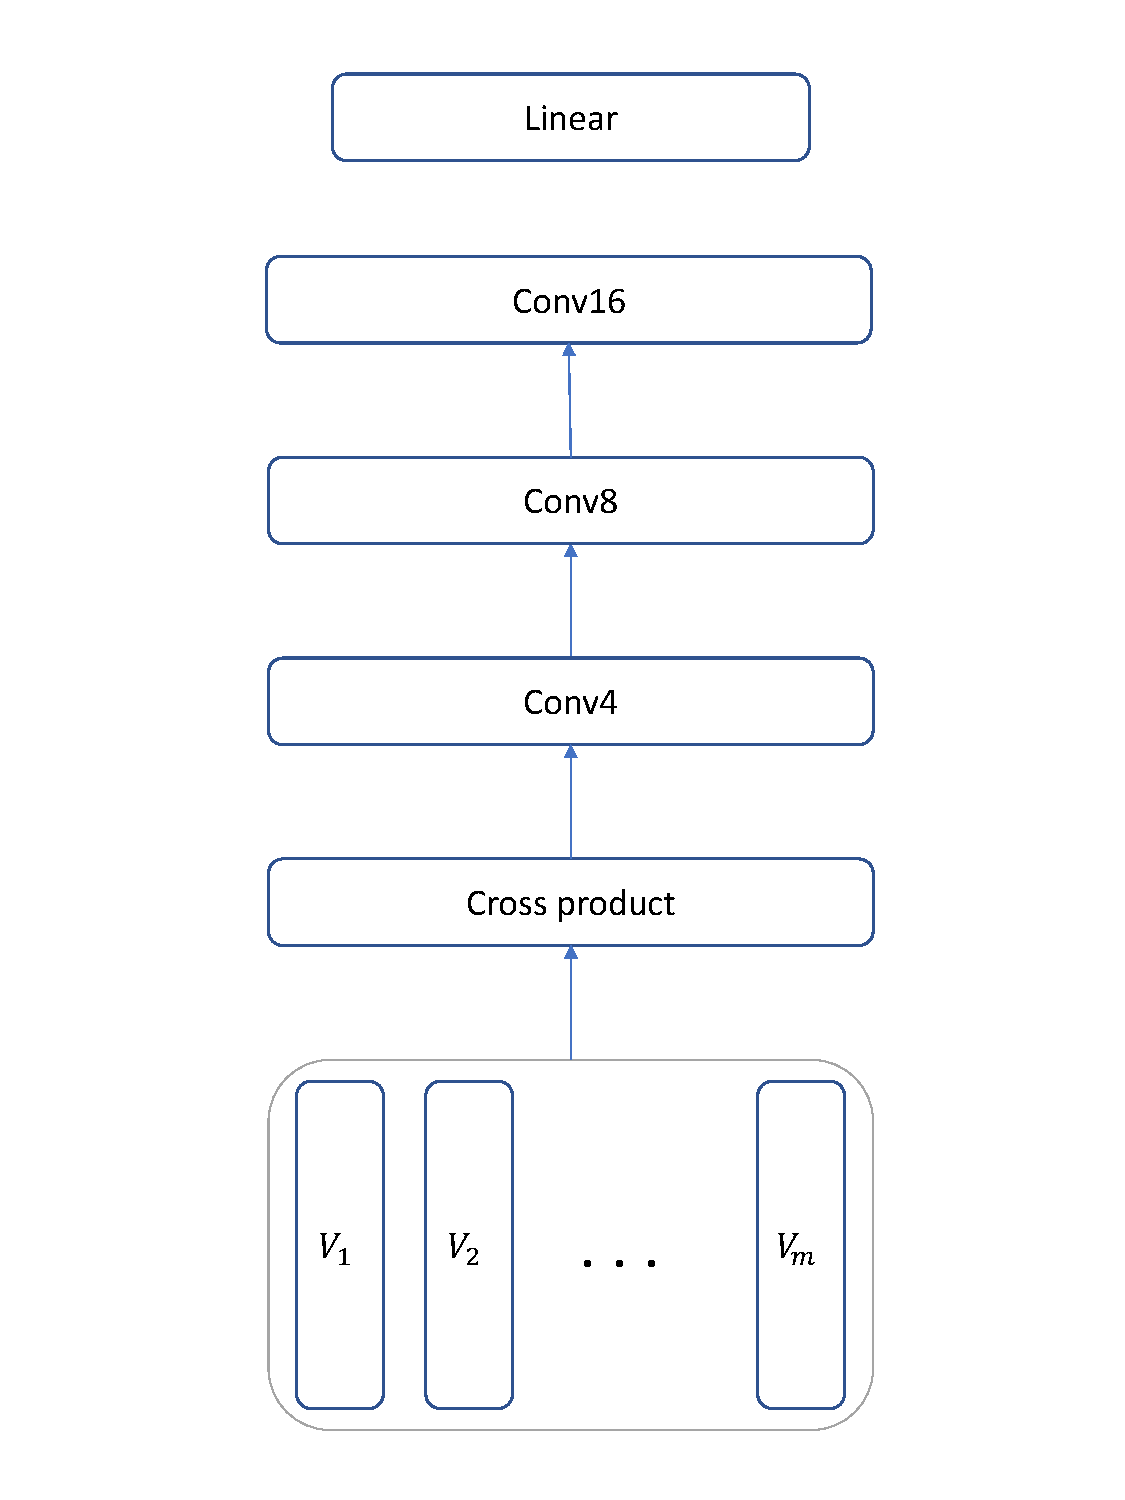
\includegraphics[width=.4\textwidth]{img/CLTN_Predicate.pdf}
    \caption{Model for Predicate}
    \label{fig:CLTN_predicate}
\end{figure}

\subsection{Universal and Existential Quantifiers}

One of the most difficult part of LTN is how to solve universal and existential quantifiers. In our implementation, we generated all the possible clause of a propositional by enumerating all variables.

For universal quantifier, the generated result is a set of clauses, while the result of existential quantifier is one clause. For example, given two propositionals $\forall \neg F(x, x)$ and $\exists y F(a,y)$, if $x,y \in {a,b,c}$, then we can get the corresponding results as $\{F(a,a),F(b,b),F(c,c)\}$ and $F(a,a)\vee F(a,b) \vee F(a,c)$

\subsection{Weighted Knowledge Base}

As we said before, we generated all possible clauses. However, such generated clauses could be even more than the observed knowledge base, which would potentially caused the overfitting on generated knowledge base and underfitting on observed knowledge base.

To solve this problem, we add a weight to each generated clause and confine that the sum of weights of clauses generated by the same propositional should equal to 1. In another word, if the generated clauses of $\phi$ is $\{\phi_1,\phi_2, \dots, \phi_n\}$, then the weight for each $\phi_i$ should be $\frac{1}{n}$.
